% !TeX root = ../main.tex

\begin{translation}
\label{cha:translation}

\title{VIR-SLAM:适用于单机器人系统和多机器人系统的视觉,惯性和测距SLAM}
\maketitle

论文出处:\cite{this}

\section{摘要}

单眼相机结合惯性测量通常可提供高性能的视觉惯性里程表。但是在较长的轨迹上,漂移可能会很明显,尤其是在视觉环
境中。在本文中,我们提出了一种系统,该系统利用超宽带测距和放置在环境中的一个静态锚点来纠正在锚点可见时的
累积误差。我们还将这种设置用于协作式SLAM:不同的机器人使用相互测距(如果可用)和公共锚来估计彼此之间的转
换,从而促进地图融合。我们的系统由两个模块组成:双层测距,视觉和惯性测距用于单个机器人,以及用于协作SLAM的
转换估计模块。我们通过模拟超宽带传感器以及真实的机器人在公共数据集上测试我们的系统。实验表明,我们的方法可
以比最先进的视觉惯性里程表高出20%以上。对于视觉上具有挑战性的环境,即使视觉惯性测距法具有明显的漂移,我们
的方法也可以使用。此外,我们几乎不需要额外的计算成本就可以计算协作式SLAM变换矩阵。


\section{引言}

机器人本地化是任何移动设备的基本主题。机器人硬件和设备的最新进展增加了机遇和需求,
多机器人系统的固有优势是高效率和鲁棒性,对于单眼相机和低成本惯性测量单元,视觉惯性里程计(VIO)被接受为
用于单个机器人状态估计的最小传感器配置和导航。考虑尺寸,重量,功率和成本\cite{delmerico2018benchmark},最
近的技术进步\cite{lupton2011visual, forster2016manifold, qin2018vins}使VIO越
来越多在许多情况下均稳定可靠。但是,漂移累积的错误造成的困难仍然很难控制。尽管闭环是系统中自然的一部分,
SLAM系统的闭环要依赖很多轨迹和环境的特殊性。例如,生成高质量的圆形轨迹需要重新访问同一位置。此外,需要
感知由照明,自相似环境等引起的异常闭环。

在本文中,我们使用单个额外的传感器(静态超宽带(UWB)锚点)来改善机器人的定位效果。 UWB近年来因其精确的测距
性能而备受关注和支持。例如,最新的苹果,撰写本文时,iPhone配备了UWB
芯片(实际上,它包括本文需要的所有传感器)。大多数可用的UWB系统使用多个(至少
4个用于3D,三个用于2D)校准锚特定区域的全球定位系统(GPS)。 这个
基础设施类型不适用于勘探未知环境,这是SLAM的主要目标目标之一。 因此,我们将系统设计为依靠
仅在一个锚点上,可以随时将其放下由机器人执行任务的形态。 我们的实验证明了这一点锚可以显着提高定位精度。


这种设置对于多机器人系统还有另一个显着的好处。多机器人SLAM是一个有前途的领域,但是
更具挑战性。 一个问题是机器人之间的转换矩阵的估计\cite{saeedi2016multiple}。 最新研究依靠共同特征提取相对姿态
,这是一种机器人内部回路闭合,得到与单个机器人循环闭合类似的约束。 一个
机器人间闭环的另一个挑战是需要交换闭环所需的信息,这很重要。
在我们的系统中,我们可以使用UWB解决这一挑战。当任何两个机器人进入各自的UWB
测距半径,他们可以相互交换测距和锚信息,他们可以估计各自的协调系统转换。有了转换矩阵,
机器人可以正确地投影所有信息,从它的邻居到它自己的坐标系。这个解决方案大大
简化了多机器人SLAM,从而最大程度地减少了需要交换功能的机器人间环路闭合的需求
数据库,闭环的识别和分布式姿势图优化。选择UWB的最后但并非不重要的原因是
数据关联的固有优势。收到距离测量值后,识别发送方的身份无需额外的努力,这将对
多机器人系统的简化提供有效的支持。此外,UWB可以在测距时提供低带宽通信。例如姿势估计可以由UWB数据包承载。未来,
我们相信单眼相机,惯性测量单位(IMU)和UWB将成文多机器人系统的标准最小配置。


\section{相关工作}


1)具有视觉惯性和测距测量功能的单机器人SLAM:SLAM一直是研究的重点
有超过三十年\cite{cadena2016past}历史。单眼视觉惯性里程计是一种流行的选择,因为它可以提供良好的状态
最少的传感器配置即可实现估算性能。尽管使用了最新的VIO算法(例如SVO [3],
VINS-Mono \cite{qin2018vins},DSO\cite{engel2017direct})在相对平移和方向上可以达到很高的精
度,累积的漂移仍然是一个问题:任何小的定向错误都可能导致较大的
端点误差。我们的系统利用UWB范围 测量以纠正累积误差。我们基于VINS-Mono开发了系统,该系统功能强大,
使用滑动窗口的多功能状态估计器视觉和IMU的紧密耦合非线性优化测量。

UWB技术本身就是一个本地化解决方案,近年来,在分米定位精度的研究和工业上有广泛应用。
但是,大多数结果是基于经过良好校准的多锚设置\cite{prorok2014accurate},不适用于在未
开发的,非结构化的环境中完成导航任务。

Wang等\cite{wang2017ultra}提出使用摄像头,IMU和UWB绕过闭环的复杂性。但是,他们仍然使用多个
预先配置的UWB锚点。他们的UWB模块提供粗略的无漂移全局位置,VIO识别本地弹道。相反,在本文中,
我们仅使用一个锚,放置在未指定的位置。 Shi等。\cite{shi2019visual}有与我们类似的思想。他们以一个UWB锚点开始,
不断从移动的机器人上抛锚。不幸,他们的实验结果仅适用于模拟EuRoC数据集的一个序列\cite{burri2016euroc},
其中有五个模拟锚点。在我们的工作中,我们专注于使用单个锚点设定。我们设计了一个双层滑动窗口算法,
有效融合准确的VIO和范围约束沿着轨迹。


\begin{figure}
  \centering
  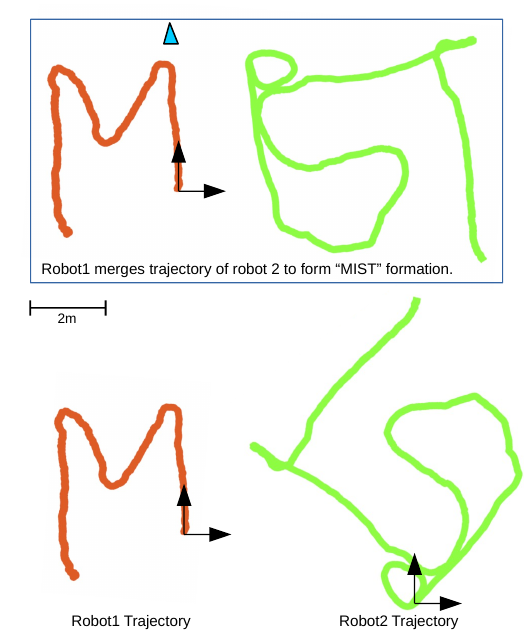
\includegraphics[width=300pt]{trans_1.png}
  \caption{两个机器人是独立手动控制的。 第一个机器人
使用Realsense T265和UWB模块时,会自己绘制一个“ M”
坐标框架。 另一台机器人搭载Realsense D435,UWB
模块和一个Pixracer飞行控制器,在其框架中绘制“ IST”。 一
将静态UWB锚放置在环境中(显示的蓝色三角形
在Robot1框架中)。 它们的轨迹显示在底部。 有两个
机器人之间的通信和测量,机器人1可以估算
来自机器人2的变换矩阵,然后在其2中映射机器人2的轨迹
顶部的图片显示了自己的框架,形成了“ MIST”(我们的实验室)。}
  \label{fig:gmapping}
\end{figure}


2)多机器人SLAM:多机器人SLAM已获得最近对提高生存能力和可达性的关注多机器人系统。 Saeedi等,\cite{saeedi2016multiple}
对多机器人SLAM进行了全面回顾,并指出了一个关键问题:相对姿态估计。最新的多机器人
SLAM系统通过分析机器人之间的环路来解决此问题关闭,可以是集中式\cite{schmuck2019ccm}或分布式
\cite{choudhary2017distributed},\cite{mangelson2018pairwise}
时尚。分布式方法更健壮,但它确实在实践中更难实现:机器人需要交换映射数据以获取要素数据库以用于将来的循环闭合,
分布式优化通常需要额外的通信和计算。测距测量可以帮助进行相对姿态估计。 Trawny等。 \cite{trawny20093d}提供理论证明和
模拟显示六个范围的测量结果用于获取两个机器人之间的转换矩阵。
Martel等。 [21]扩展工作并将其适应于4DOFUWB设置的相对姿态估计,并将其用于
为VR应用程序合并地图。两种方法的使用范围长轨迹的测量。在我们的解决方案中,机器人可以尽快估算出转换矩阵
从邻居那里得到两个测量值实时转换估计的要求机器人会合。这两种方法\cite{trawny20093d},\cite{molina2019unique}代表
当没有公共锚点并且可以与机器人之间的闭环相结合,以改善转换结果。

实际上,大多数文学作品都探索了具有视觉和/或多个UWB锚点的组合IMU。在本文中,我们专注于单个锚点的使用
在任意位置,这很容易部署为信标在实际的勘探任务中。我们建议双层滑动结合VIO和UWB测距的窗口技术
利用VIO产生无漂移状态估计由于其准确的短时相对姿态估计,以及范围约束,以延长轨迹。此外,记录
锚定范围可以帮助机器人找到转换矩阵在多机器人中仅需进行两次距离测量即可高效设置。我们的贡献可以总结为:

\begin{itemize}
	\item 用于单个机器人的UWB辅助SLAM系统,优于最新的VIO;
	\item 结合了双层滑动窗口算法通过VIO和UWB测距进行相对姿态估计约束
	\item 估算多个机器人之间的转换矩阵的有效方法。
\end{itemize}


\section{系统设计}

在本节中,我们解释了预备符号和符号在本文中使用。 然后,我们详细介绍我们的公式
测距辅助视觉惯性SLAM,着重于成本优化问题的因素。 最后,我们介绍我们用于估计变换矩阵的解决方案
机器人之间。


\begin{figure}
  \centering
  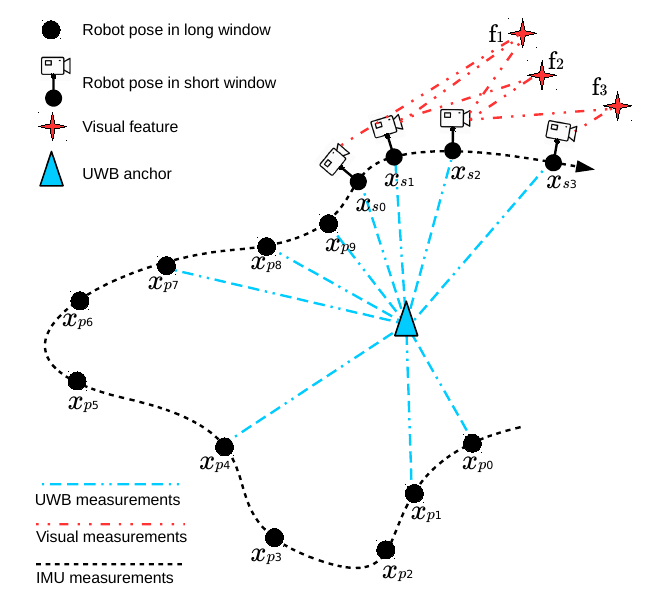
\includegraphics[width=300pt]{trans_2.png}
  \caption{ 具有单个锚点的VIR-SLAM方案的图示
设定。 来自传感器的测量值以不同的线显示。 机器人
相机的姿势和IMU测量值属于短滑
窗口。 保留与UWB相关联的所有姿势以锚定
长的滑动窗口。}
  \label{fig:gmapping}
\end{figure}


\subsection{单机器人估计}


我们假设机器人携带三种传感器(单眼相机,IMU和UWB模块)并移动在3D环境中,如图2所示。UWB锚点是
放置在初始位置未知的环境中。我们将机器人i的世界框架定义为$[]^{iw}$,即通常在机器人与第一个相机镜框对齐时
开始执行任务。锚的位置表示在机器人世界框架中,用$P_{iw}$表示一个 。我们使用$[]^{ib}$表示机器人i的身体框
架,类似地$[]^{ic}$相机镜框。请注意,我们没有定义UWB传感器帧,因为它是标量测量。超宽带测距考虑到
UWB天线在车身框架中的3D偏移。经典VIO提出了以下方面的优化公式,在大小为n的滑动窗口上的状态为:

\begin{equation}
  X = [x_0, x_1, ..., x_n, l_0, l_1, ..., l_m] \\
    x_k = [p_{b_k}^{iw}, v_{b_k}^{iw}]
\end{equation}

其中包括所有n帧的状态x和视觉 特征反深度l。第k帧状态$x_k$包括 位置$p_{b_k}^{iw}$速度$v_{b_k}^{iw}$
以及四元数的方向$q_{b_k}^{iw}$ 适用于机器人i及其世界范围内的加速度计 偏差$b_{a_k}^{ib}$
和陀螺仪偏置b ib 周 在它的身体框架中。里 是m个特征中第i个特征的反深度 从滑动窗口上的视觉观察。如果
滑动窗口包括自 任务的开始,优化就变得完整了 平滑估计。尽管完全平滑提供了 最佳精度,实际上是不可扩展的,
因此我们使用一个密钥 丢弃相似帧而又不会丢失的帧方法 跟踪。但是,随着轨迹变长,尺寸 的国家不断增长。因此,我们确定密钥的大小
框架并将旧的关键框架边缘化为先验因素。

在优化中。 视觉惯性里程表的漂移 仍然很难避免,并且使用循环进行姿势图优化 关闭成为纠正累积的唯一机会
错误。 瞄准准确的本地化系统并避免 都依赖于闭环,我们设计了一个SLAM系统, 使用新颖的双层推拉窗结构,
基于VINS-Mono的实现[4]。


\begin{figure}
  \centering
  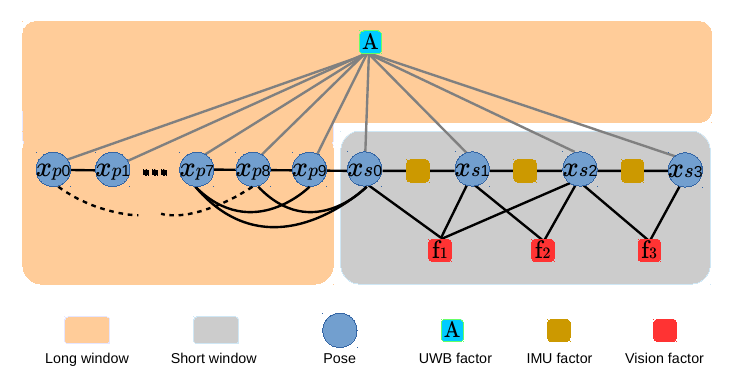
\includegraphics[width=300pt]{trans_3.png}
  \caption{图2中场景的因子图。因子图包括
姿势,UWB因子,IMU因子和视觉因子。 边缘是错误。
对于范围测量的姿势,我们有一个UWB因子。 进一步,
姿势之间添加了平滑的边缘(曲线)。}
  \label{fig:gmapping}
\end{figure}


\subsection{双层紧连接的VIR优化}

我们提出了一个紧密耦合的双层滑动窗 通过考虑以下方面来优化SLAM:高 来自VIO的准确相对姿态估计,较不准确
但是绝对的UWB测量和计算成本 对于这些因素。 我们设计了两个滑动窗,涉及三种 变量,如等式所示。 2.短窗口Ψ,与
尺寸为n的经典可视SLAM滑动窗 等式1。此窗口中的变量包括xk(等式3)和 $[l_0,l_1,... ,l_m]$,其含义与
等式1.我们系统的新颖之处在于增加了 另一个长滑动窗口carries带有状态wt 如方程式所示。 4.长滑动窗口的大小为s,
比n大得多仅此窗口中的状态 包含机器人位置$p_b^{iw}$在机器人世界框架中。

\begin{equation}
    X = [w_0, w_1, .. , w_s, x_0, x_1, ..., x_n, l_0, l_1, ... , l_m]
\end{equation}


图3显示了我们系统的因子图,对应于 图2的场景。灰色的短窗口区域包括 摄像机和IMU测量的状态。长
橙色的窗口区域包含UWB的状态 测量。根据状态定义,我们制定 完全非线性优化问题为:

\begin{equation}
  \min\limits_{X} \{ \sum\limits_{x \in \Omega} \rho(||r_u(z_t, X)||_{P_{b_t}^{iw}}) +
    \sum\limits_{k \in \Phi} ||r_B(z_{b_{k+1}}^{b_k}, X)||^2_{P_{b_{k+1}}^{b_k}} +
    \sum\limits_{(i,j) \in C} \rho (||r_C(z_l^{c_j}, X)||^2_{P_l^{c_j}})
  \}
\end{equation}

此非线性优化问题考虑了三个因素,分别对应于UWB因子,IMU因子和 视觉因素。 UWB残差是针对
长窗window,而IMU和视觉残差为短 窗口$\phi$。

1)UWB因素:UWB本地化使用不同的协议:到达时间(TOA),到达时间差 (TDoA)和双向测距(TWR)。在我们的系统中
我们使用TWR,它测量两个之间的距离 收发器通过来回发送数据包。虽然 受支持的节点数量有限,原因是 共享的UWB
通信介质,可以使用TWR 没有设备同步,这使得协议 广泛使用。由于我们没有考虑数百个 机器人同时通讯,我们选择TWR
避免同步,这可能很难实现 在分布式多机器人应用中。我们为测距建模 UWB模块的测量结果为:

\begin{equation}
    d = d + b_d + e
\end{equation}


其中ˆd是UWB测量值,d是真实距离,bd是 基于距离的偏差,e是跟随高斯的误差 分布N(0,σ2
)。请注意,bd可以使用 通过预先收集数据来预先建立一个高斯过程模型 基本事实。然后可以将模型简化为:

\begin{equation}
ˆd = d + e
\end{equation}

通过这种简化的UWB模型,我们定义了UWB因子 在Equ。 5为:


\begin{equation}
    r_u(z_t, X) = r_r * \rho(||p_{b_t}^{iw} - P_{A}^{iw}|| - d_t)
\end{equation}

上面的UWB因子包括两个残差: 测量残差和虚拟相对转换 测量残差。 γr和γs是它们的权重
两个残差。 ˆdt是UWB测距, 与机器人预测的范围进行比较 车身框架t到锚点Piw 世界框架中的A。至
避免范围因素过度影响优化器 并打破视觉惯性的相对姿势属性 估计,我们引入虚拟相对变换 测量ez
在帧t和j∈(t,t + s]之间 从短滑动窗口估计结果中提取。 我们在实验中选择s = 3来创建两个连续的

姿势之间的链接,例如
在图3中$\rho()$是一个伪Huber损失函数,定义为$ \rho (q)= \delta 2( p_1 +( q /\delta) 2-1)$。

2)IMU因子:IMU测量对于 单眼视觉测距法。作为IMU的频率 通常高于相机的图像帧速率,IMU
在两个连续的测量之间预先集成了测量 图像帧[2]。通过参考最后的身体框架运动, 该技术可避免重复的IMU重新整合并减少
优化过程中的计算。福斯特等。 [3]扩展这个 So3旋转群So3的歧管结构的方法 更高的准确性和鲁棒性。我们遵循相同的方法
如四元数形式的[4]。 在bk和bk + 1的两个连续帧之间参考帧bk的预集成IMU测量值可以是
aˆt和ωˆ t是加速度计和陀螺仪的测量值 向量。这三个公式对应于位置,速度和方向的相对运动变化
到bk的局部身体框架。 IMU因子是预测运动之间的残差 以及与车身框架有关的预积分结果:
是参考的估计位置,速度和方向
到bk的局部主体框架(有关详细信息,请参见[4])。

\begin{figure}[H]
  \centering
  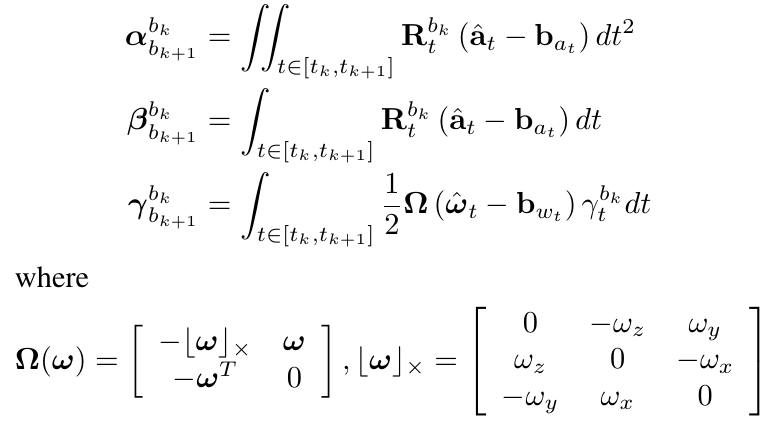
\includegraphics[width=300pt]{trans_equ1.png}
  \caption{}
  \label{fig:gmapping}
\end{figure}

3)视觉因素:视觉因素包括被跟踪要素的重投影误差。我们使用策略 与[4]相似,比较了
当前框架及其最初的观察结果。我们定义 视觉残差为 是图像中特征lk的坐标
相机框架j的π()是转换为 将齐次坐标转换为图像坐标R cj
词 T cj 词 表示帧变换(旋转和平移

从相机框i到j从状态推断 姿势,和P 词 lk 是第k个要素在 第一观察架视觉因素通过 估计的所有帧和所有跟踪的特征
州。

4)锚点位置估计:在以上讨论中,我们假设锚点坐标可用于优化程序。由于锚位置是
最初未知,需要估计。因此,开始时要估计的状态向量变为

\begin{equation}
X = [P_{iw} A, w_0, w_1, ..., w_s, x0, x1, ... , x_n, l_0, l_1, ... , l_m]
\end{equation}

成本函数和因子保持不变。的 Piw的优化结果 初始化阶段之后是 保存为固定值。我们用
两个注意事项:a)锚在实践中是静态的, b)通常,初始化阶段可以控制 然后机器人在锚点附近移动。虽然
距离测量误差与 距离值,锚位置的估计取决于 在远处。换句话说,轨迹长度之比 初始化中的距离会影响估计。
因此,我们将初始估计值视为固定值。 C.分布式协作SLAM 我们的测距辅助系统的另一个显着优势是 有了一个
共同的锚点,机器人就可以直接估算 机器人之间的交会时,它们会合。机械人 仅需在对邻居进行测距时发送其
当前位置和锚位置。收到这个之后 信息两次,机器人可以计算出转换 自身与发送者之间的矩阵。一旦转型
正确估计矩阵,从 邻居可以正确放置在机器人的框架中。 估计机器人之间的转换是多机器人系统的关键要求。我们标记
将坐标系从机器人i转换为j 是3×1的翻译向量。随着 借助加速度计和陀螺仪,我们可以建立
方向,并为所有机器人定义相同的z轴。 VINS-Mono使用相同的策略:z轴对齐 创建坐标时与重力相反
系统。因此,仅偏航角θ和3D偏移t 使用两个机器人的锚点位置估算, 我们可以很容易地得到$tz = (P w A-w A)z$
,即 差向量在z轴上的投影。这离开 估计三个参数(θ,tx,tz)。 图4显示了如何估计其余参数。
让我们假设两个机器人i和j在 2D为简单起见(不失一般性,就像我们已经 知道z轴偏移tz)。


\begin{figure}
  \centering
  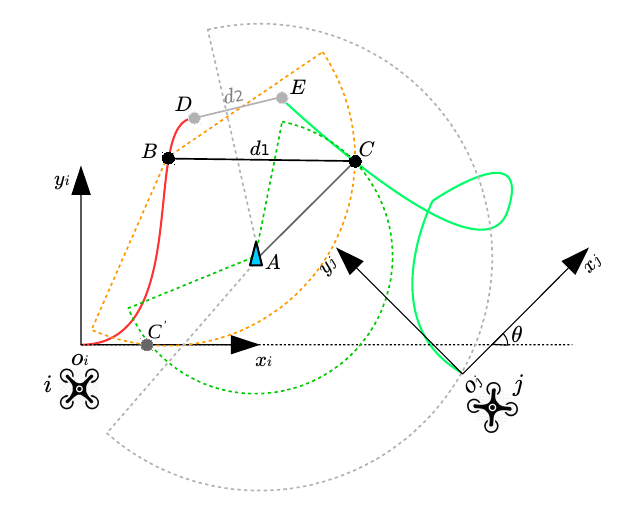
\includegraphics[width=300pt]{trans_4.png}
  \caption{多机器人场景的变换矩阵估计。}
  \label{fig:gmapping}
\end{figure}

两个机器人都有自己的
坐标系oixiyi和ojxjyj。他们也有 初始化后定位一个位置,并拥有自己的位置 在各自坐标系中跟踪的轨迹。
当机器人i通过B点而机器人j通过C点时, 他们进入通讯范围,他们都可以 相互距离测量值d1。同时,他们
传送他们的当前位置和A的位置( 在自己的坐标系中)。 我们以机器人i的观点来说明我们的解决方案。什么时候
机器人i接收锚点的位置和当前 机器人j的位置(点C),以j的框架P表示
, 分别。然后,机器人我知道了ojxjyj的起源 必须位于锚点周围带有半径的灰色圆圈上
找到机器人j的位置C必须位于 半径为| AC |的A周围的绿色圆圈。众所周知, B点和C点之间的距离是范围测量
d1,C点也必须位于其周围的橙色圆圈上 当前位置B,半径为d1。 因此,当前位置位于绿色和橙色圆圈C和C之间的交点之一
0
。寻找 哪个路口如果正确,我们再加一个 在随后的两个点D和E之间测量d2。 按照相同的步骤,我们可以找到候选人
为清楚起见,我们没有为D和 E.通过比较E,E0之间的关系 ,C和C 0与
从C到E的真实运动,我们可以找到C并确定 转变钛
在哪里
Q
表示点Q中的3D位置矢量
机器人的世界坐标系

\section{实验}

\begin{figure}
  \centering
  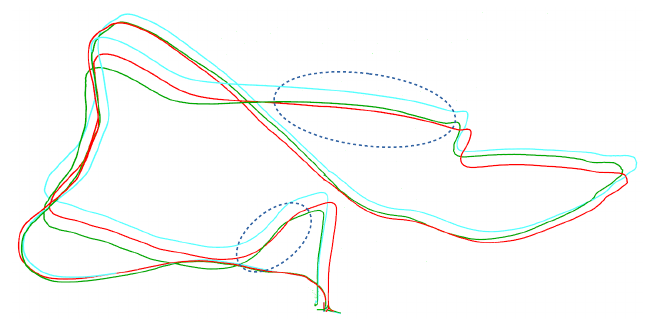
\includegraphics[width=300pt]{trans_5.png}
  \caption{VIR在EuRoC MH05数据集上的表现。 我们方法的ATE错误是
0.291m,相比之下,VINS-Mono MONO(0.388m)。 我们设置的方法在大多
数部分中更接近于地面事实,这证明了校正漂移误差的存在。}
  \label{fig:gmapping}
\end{figure}


我们使用公共数据集验证算法,并进行了真正的硬件实验。 我们选择VINS-Mono1,和TUM评估工具进行比较2
。我们计算 地面真值的绝对轨迹误差(ATE) 可用。对于我们的大面积实验,我们计算始端误差。 

A.EuRoC数据集实验 我们在EuRoC [15]数据集上测试了单个机器人跟踪系统。
我们从地面真实数据模拟UWB测距。假定静态锚点 在机器人初始化期间创建的框架的原点。
我们添加高斯白噪声N(0,0.05)来模拟误差 我们的UWB传感器。 VINS-Mono的滑动窗口大小
设置为10。对于我们的系统,我们用一个短窗口进行了测试 大小为10,长窗口大小为100。 表一显示了我们的VIR-SLAM在性能上胜过VINS-Mono
ATE条款。举例来说,我们展示了 图5中EuRoC MH-05序列的比较。的 我们方法的绿色轨迹更接近红色地面
真相。从椭圆指标,我们可以看到我们的估计 即使在漂移时也可以纠正错误。 B.单机器人实验
我们还使用带有真实UWB的Spiri机器人测试了系统 传感器,如图6所示。该系统具有D435 Realsense 相机,但我们将其用作单眼相机。 IMU
测量来自Pixracer飞行控制器,并且 该机器人携带Nvidia TX1作为车载计算机。我们 



\begin{figure}
  \centering
  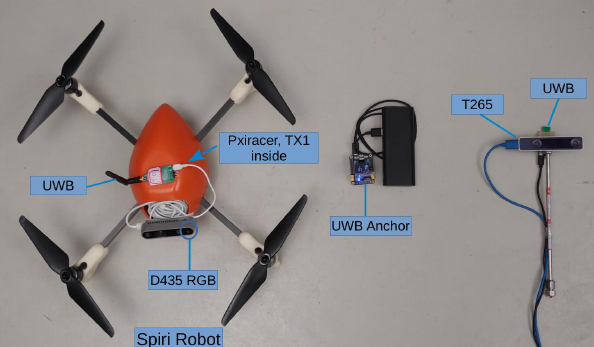
\includegraphics[width=300pt]{trans_6.png}
  \caption{对于单机器人实验,我们使用Spiri机器人(带Pixracer
和NVIDIA TX1)。 我们添加了Realsense D435相机(尽管我们仅
使用RGB)和UWB传感器模块。 IMU测量值
来自Pixracer。 Realsense T265在
右侧,在我们的多机器人实验中模拟了第二个机器人。}
  \label{fig:gmapping}
\end{figure}

\begin{figure}
  \centering
  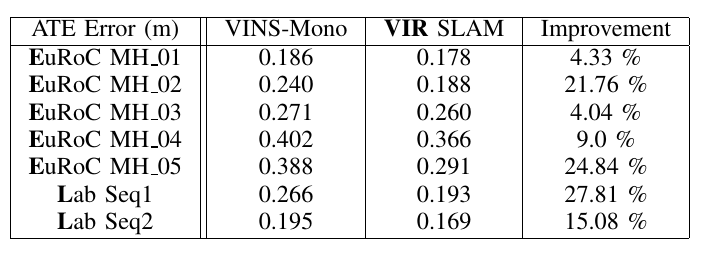
\includegraphics[width=300pt]{trans_table1.png}
  \caption{表I}
  \label{fig:gmapping}
\end{figure}

B. 使用OptiTrack运动捕捉。在我们的实验室中测试系统作为基本事实,我们手动控制机器人并收集两个序列:
结果列于表I。为清楚地看到两者之间的区别, 我们显示了相同来源的轨迹。这不一样 从对齐两个轨迹来计算ATE。如
如图7所示,我们的估计器的累积误差小于 酒单。 我们还测试了大型中庭的系统性能。的 中庭的环境充满挑战:毫无特色
墙壁,光线不足的条件,带有反射的玻璃墙等。 我们围绕中庭移动机器人,并确保机器人 在开始的同一点结束。然后我们
比较开始到结束的错误。如图8和表II所示,VINS-Mono 估计有很大的漂移,超过5.4m。虽然
闭环版本可以纠正漂移,因为循环 检测到闭合,轨迹中仍然存在明显的错误。 但是,我们的VIR SLAM可以正常工作,没有任何循环
关闭。起点和终点有一个小的二维误差(0.148m),但我们的系统引入了更大的误差:z轴上的累积误差。我们认为这是由于
锚点靠近机器人的水平面,并且 测量的微小差异无助于纠正 z坐标。我们手动检查了UWB测距
沿上下边缘的信息,我们可以 确认我们的估计值在合理范围内。


\begin{figure}
  \centering
  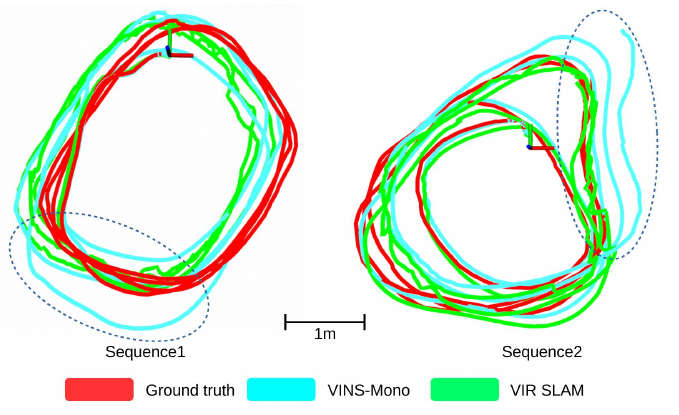
\includegraphics[width=300pt]{trans_7.png}
  \caption{使用OptiTrack地面实况进行的VIR室内实验。 左边和
正确的数字是两个序列。 所有轨迹都从原点开始,并且是
不对齐的。实验显示我们的估算器不会出现过多的漂移。}
  \label{fig:gmapping}
\end{figure}



C.多机器人实验。我们还测试了我们的多机器人技术,如图1所示。 我们手动独立控制两个机器人来制造
类似于我们实验室名称“ MIST”的轨迹。 我们 在环境中放置一个静态UWB锚点。 首先 机器人暗示Realsense T265和UWB模块
在图6(右)中。 我们将其移动以形成“ M”形。 的 另一个机器人Spiri沿“ IST”运动,并受到控制 独立地。 他们在每个机器人框架中的轨迹是
如图1的底部所示。仅使用两个机器人间 测量(通过数据交换),机器人1可以估算 机器人2的变换及其地图机器人2的轨迹
自己的框架,如图1顶部所示。


\begin{figure}
  \centering
  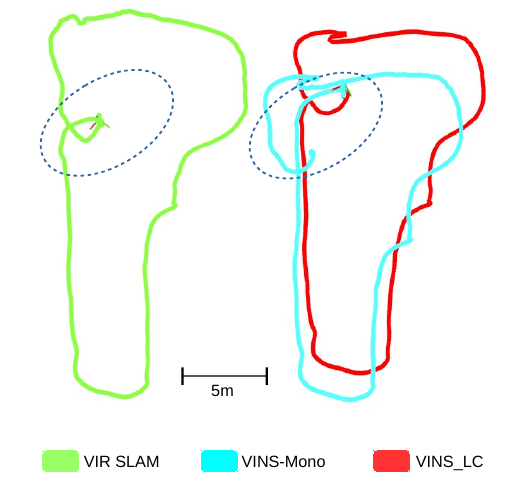
\includegraphics[width=300pt]{trans_8.png}
  \caption{}
  \label{fig:gmapping}
\end{figure}


\section{总结}

在本文中,我们提出了一种新颖的SLAM:VIR-SLAM,它结合视觉,IMU和UWB传感器。 通过
在环境中任意设置静态UWB锚,机器人可以进行无漂移状态估计。 我们的解决方案结合了准确
VIO的相对姿态估计,并修正了累积误差。我们的实验 显示,引入的静态锚点可以帮助纠正漂移,
有效地提高了定位精度。 我们还展示了一个示例,其中两个独立的机器人分别映射在获得两个后,
另一个机器人到自己坐标的轨迹
范围测量。 这种技术可以完成机器人到机器人之间的转换,这对于多机器人SLAM意义重大。


\nocite{abrahams99tex,salomon1995advanced}
\bibliographystyle{plainnat}
\bibliography{ref/appendix}

% 也可以使用 thebiliography 环境手写
\begin{thebibliography}{2}    

  \bibitem{this}
Cao, Y., & Beltrame, G. (2020). VIR-SLAM: Visual, Inertial, and Ranging SLAM for single and multi-robot systems. arXiv preprint arXiv:2006.00420.

  \bibitem{delmerico2018benchmark}
  J. Delmerico and D. Scaramuzza, “A benchmark comparison of
monocular visual-inertial odometry algorithms for flying robots,” in
2018 IEEE International Conference on Robotics and Automation
(ICRA). IEEE, pp. 2502–2509.

  \bibitem{lupton2011visual}
  T. Lupton and S. Sukkarieh, “Preintegration visual-Inertial-Aided
Navigation for High-Dynamic Motion in Built Environments Without
Initial Conditions,” IEEE Transactions on Robotics, vol. 28, no. 1, pp.
61–76, Feb. 2012.

  \bibitem{forster2016manifold}
 C. Forster, L. Carlone, F. Dellaert, and D. Scaramuzza, “On-Manifold
Preintegration for Real-Time Visual–Inertial Odometry,” IEEE Trans-
actions on Robotics, vol. 33, no. 1, pp. 1–21, Feb. 2017.

  \bibitem{qin2018vins}
T. Qin, P. Li, and S. Shen, “VINS-Mono: A Robust and Versatile
Monocular Visual-Inertial State Estimator,” IEEE Transactions on
Robotics, vol. 34, no. 4, pp. 1004–1020, Aug. 2018.

  \bibitem{5}
 “Loco Positioning system | Bitcraze.” [Online]. Available: https:
//www.bitcraze.io/loco-pos-system/


  \bibitem{saeedi2016multiple}
 S. Saeedi, M. Trentini, M. Seto, and H. Li, “multi robot slam review
Multiple-Robot Simultaneous Localization and Mapping: A Review,”
Journal of Field Robotics, vol. 33, no. 1, pp. 3–46, 2016.



  \bibitem{cadena2016past}
C. Cadena, L. Carlone, H. Carrillo, Y. Latif, D. Scaramuzza, J. Neira,
I. Reid, and J. J. Leonard, “Past, present, and future of simultaneous
localization and mapping: Toward the robust-perception age,” IEEE
Transactions on Robotics, vol. 32, no. 6, pp. 1309–1332, 2016.


  \bibitem{engel2017direct}
J. Engel, V. Koltun, and D. Cremers, “Direct Sparse Odometry,” IEEE
Transactions on Pattern Analysis and Machine Intelligence, vol. 40,
no. 3, pp. 611–625, Mar. 2018.

  \bibitem{prorok2014accurate}
A. Prorok and A. Martinoli, “Accurate indoor localization with ultra-
wideband using spatial models and collaboration,” The International
Journal of Robotics Research, vol. 33, no. 4, pp. 547–568, 2014, 05.

  \bibitem{wang2017ultra}
M. W. Mueller, M. Hamer, and R. D’Andrea, “Fusing ultra-wideband
range measurements with accelerometers and rate gyroscopes for
quadrocopter state estimation,” in 2015 IEEE International Conference
on Robotics and Automation (ICRA). Seattle, WA, USA: IEEE, May
2015, pp. 1730–1736.


  \bibitem{shi2019visual}
X. Fang, C. Wang, T.-M. Nguyen, and L. Xie, “Graph Op-
timization Approach to Localization with Range Measurements,”
arXiv:1802.10276 [cs], Feb. 2018, arXiv: 1802.10276.

  \bibitem{wang2017ultra}
C. Wang, H. Zhang, T.-M. Nguyen, and L. Xie, “Ultra-wideband aided
fast localization and mapping system,” in 2017 IEEE/RSJ International
Conference on Intelligent Robots and Systems (IROS). IEEE, 2017,
pp. 1602–1609.


  \bibitem{shi2019visual}
Q. Shi, X. Cui, W. Li, Y. Xia, and M. Lu, “Visual-UWB Navigation
System for Unknown Environments,” p. 11.


  \bibitem{burri2016euroc}
 M. Burri, J. Nikolic, P. Gohl, T. Schneider, J. Rehder, S. Omari, M. W.
Achtelik, and R. Siegwart, “The EuRoC micro aerial vehicle datasets,”
The International Journal of Robotics Research, vol. 35, no. 10, pp.
1157–1163, Sep. 2016.


  \bibitem{saeedi2016multiple}
 S. Saeedi, M. Trentini, M. Seto, and H. Li, “Multiple-Robot Simultane-
ous Localization and Mapping: A Review,” Journal of Field Robotics,
vol. 33, no. 1, pp. 3–46, 2016.


  \bibitem{schmuck2019ccm}
P. Schmuck and M. Chli, “CCM-SLAM: Robust and efficient central-
ized collaborative monocular simultaneous localization and mapping
for robotic teams,” Journal of Field Robotics, vol. 36, no. 4, pp. 763–
781, 2019.


  \bibitem{choudhary2017distributed}
 S. Choudhary, L. Carlone, C. Nieto, J. Rogers, H. I. Christensen,
and F. Dellaert, “Distributed Mapping with Privacy and Communica-
tion Constraints: Lightweight Algorithms and Object-based Models,”
arXiv:1702.03435 [cs], Feb. 2017, arXiv: 1702.03435.


  \bibitem{mangelson2018pairwise}
 J. G. Mangelson, D. Dominic, R. M. Eustice, and R. Vasudevan,
“Pairwise consistent measurement set maximization for robust multi-
robot map merging,” in 2018 IEEE International Conference on
Robotics and Automation (ICRA). IEEE, 2018, pp. 2916–2923.


  \bibitem{trawny20093d}
 N. Trawny, X. S. Zhou, and S. I. Roumeliotis, “3d relative pose
estimation from six distances.” 2009.


  \bibitem{molina2019unique}
F. M. Martel, J. Sidorenko, C. Bodensteiner, M. Arens, and U. Hugen-
tobler, “Unique 4-DOF Relative Pose Estimation with Six Distances
for UWB/V-SLAM-Based Devices,” Sensors, vol. 19, no. 20, p. 4366,
Oct. 2019.

\end{thebibliography}


\end{translation}
